\chapter{Solution}
\label{solution}
\lettrine[lraise=0.1, nindent=0em, slope=-.5em]{\color{Violet}T}{he} solution chapter is divided into four parts. First, the design phase uses information gathered from analysis phase of the \gls{ADDIE} process and the main goals are identifying  a learning objectives, compose tests, choose course format, and planning of the learning process~\citep{website:design_phase_ADDIE}. Second, the technical implementation of the e-learning course is usually a sub-part of the previous part a design process of the \gls{ADDIE} model. However, the section focusing to the technical considerations, deserve separate part according to context of this e-learning course because its importance and capacity. Third, a development phase describes authoring of the learning material. Fourth, the implementation phase covers piloting of the course, where each part of the course are run-through with particular students/trainers to get feedback about timing, content and ~\citep{website:design_phase_ADDIE}.



 
\section{Design and Planning of learning process}
The Design phase contains four steps: First, design of the learning objectives; Second, design the assessments for each objective. Third, choose a course format. Fourth, create an instructional strategy~\citep{website:design_phase_ADDIE}. However, in this thesis, the tests are designed together with the learning objectives to simplify reading the topics.

\subsection{Design of the course content and learning objectives}

In the analysis phase a learning outcomes were established. For design an adequate course content two aspects are required, learning objectives and assessment tests. Likewise in software development field the tests should be designed first to ensure creation of consistent learning materials and labs. Therefore all learning objectives are given with evaluation methods and values.  

The terms and topics used in assessment should stay on level the students should know at the end of the lab and derived from learning objectives established in analysis phase.

Developed tests and materials of the course will be listed in course syllabus~\ref{Course Syllabus}.

\subsubsection{Pre-requirements courses}

During the analysis of the target group the need for preliminary course was decided to homogenize a knowledge and a skill level of the participants.

The objectives and assessments for preliminary course:
\begin{itemize}
\item Student are able to work with command line using GNU/Linux and are able: working with files, manage software, manage disks and partitions, manage users and groups, configure networks and user's login session. Minimal level for pass is to gain more then 50\% of randomly chosen test version, included in Appendix~\ref{Preliminary Tests} in Table~\ref{tab:preliminary_practical_test}
\item Student are able to explain basic terminology of operating systems sush as: kernel, GUI, shell, Virtual memory, authentication, authorization, RAM, cache, buffer, latency, throughput, file system, process, thread, password hash, DAC, MAC, RBAC, command parameter, command flag, file system hierarchy, environment variable). Minimal level to pass is gather more then 51\% of closed book test like in sample in Appendix~\ref{Preliminary Tests}
\item Student are able to configure a network of the GNU/Linux and explain terms like gateway, netmask, IP address, port, IP alias, DNS servers. Minimal level to pass is successful configuring network for lab machines.
\item Student is able to read/modify and create simpler BASH, Python and PowerShell scripts. Minimal level of pass is create script with all common language construction in one particular language. Powershell scripting is included because furtherer labs contains also integration labs with Active Directory, SAMBA4, GNU/Linux servers and workstations and Windows workstations.
\end{itemize}

According to previous objectives six practical classes are needed:\footnote{All times are given in academic hours or days which equal 8 academic hours.}

\begin{enumerate}[label=LAB \arabic*.,leftmargin=*]
\item Operating system basics (one day)
\item Basic networking IPv4/IPv6, TCP/IP (one day)
\item GNU/Linux basics (and OpenBSD/FreeBSD basics) (16h) as describbed in Appendix~\ref{Preliminary course - dpkg based GNU/Linux} on page~\pageref{Preliminary course - dpkg based GNU/Linux}
\item Scripting in BASH (2 days)
\item Scripting in Python (1.5 days)
\item Scripting in PowerShell (1.5 days)
\end{enumerate}
After implementing the course exact load is known numbers will be arranged.

\subsubsection{Root Services}
In this particular case the term root services are described as \gls{NTP}, \gls{DNS}, \gls{DHCP} services.
After finishing this lab block the student are able to configure root services and use those services in furtherer labs.
The objectives and assessments for Root Services lab:
\begin{itemize}
\item After finishing this lab student is able to install \gls{NTP} service on the server and on the client computer and configure client to use internal server (pool) and server to use upstream \gls{NTP} service and fall-back services. Minimal level to pass: Services are configured, and student demonstrates debug skills with different tools and user explains basic terms and (pool, stratum, delay , offset, jitter, drift)
\item After finishing this lab student is able to install \gls{DNS} service and configure clients for new server. Minimally, students are able to configure zones, reverse zones, master -- slave replica, forwarding, different type of records (like MX, A, CNAME, TXT for SPF, PTR) and use basic management utilities to do following tasks: reload zone, flush name, flush cache, add records dynamically, freeze and thaw zones). Configured service should able to do recursive quires for one particular subnet and student are able to explain what DNS attacks are common in Internet and what is an Open Resolver. Student tests nameserver of the \gls{EITC} and explains what is wrong with that.
\item After finishing this lab student is able to install \gls{DHCP} server and configure hosts using this service. Minimal level for pass: Student installs and configures service what gives networking configuration to client machine from range or using hardware address. Service updates \gls{DNS} records using shared key (Mandatory Access Control must not disabled for pass)
\end{itemize}
According to previous objectives three practical classes are needed:
\begin{enumerate}[label=LAB \arabic*.,leftmargin=*]
  	\item NTP (4h)
  	\item DNS (2.5 days)
  	\item DHCP (one day)
\end{enumerate}

\subsubsection{Web and File services}
Configuring and securing web servers is essential skill required from system administrators. Therefore, web server installation, configuration and hardening are covered in this block.

The learning objectives and assessments for Web and File services:
\begin{itemize}
\item After completing the web and file services block student is able to install web server and web application with database and several virtual hosts and configure \gls{TLS}. Minimal level for passing: Installed web server with two virtual hosts accepting \gls{HTTP} and \gls{HTTPS} connections. Configured IP aliases for \gls{HTTPS} and/or \gls{SNI}.
\item Student is able to use caching technologies to protect web application against simpler \gls{DOS} attacks. Student configures web service and demonstrates that installed application can be easily taken offline using a simple load generator. Thereafter, the student configures web application accelerator as mitigation method against the  \gls{DOS} attack. Minimal level: Student configures proper caching and demonstrates that web application survives same attack.
\item Student are able to install different application firewalls as \gls{SQL} firewall and web application firewall. Minimal level: Student demonstrates that different types of attacks are possible and successful against the vulnerable web application. Student installs \gls{SQL} firewall and demonstrates that basic \gls{SQLi} attacks are blocked. Student demonstrates that several web application attacks are still possible after installing the \gls{SQL} firewall as reflected \gls{XSS} and stored \gls{XSS}, command injection and \gls{CSRF}. Student installs application firewall before web application and demonstrates that previously succeeded attacks (at least \gls{XSS}) are stopped.
\item Student is capable to install file server and configure shares, permissions, groups. Criteria: Student installs the service and configures two shares and group based permissions for each share. Student configures client machine to mount one share when user logs on and other share should mounted on boot.
\end{itemize}


According to previous objectives four practical classes are needed:
\begin{enumerate}[label=LAB \arabic*.,leftmargin=*]
   \item Web server basics - installation and configuring web server (4h)
  	\item Web server security - Protecting Web Application Against (D)DOS Attacks (6h)
  	\item Web server security - securing vulnerable web application using application firewalls (6h)
  	\item Fileserver installation and configuration (4h)
\end{enumerate}


\subsection{Choosing the course format}

For developing e-learning courses a choosing course format have a big influences to all participants \citep[p.14]{OppeArenduskeskus2010}. 

Common course delivery formats used in e-learning and blended learning (combined form of instruction-led and e-learning) used in \gls{EITC} are: 
\begin{itemize}
\item Asynchronous e-learning - \gls{SIS}, wikis, \gls{LMS}'s, forums, blogs and other collaboration systems.
\item Synchronous e-learning - virtual distance laboratories, remote access for some servers, Skype and other online communications.
\item Instructor-led lessons - practical classes
\item Self-study - homework, reading books and other resources.
\end{itemize}

For this course several methods are used in different cases. First, a self-study are possible because all materials are available from web (except some video materials) in most cases all virtual machines are also publicly downloadable and participants may self-study. Second, combining self-study and instruction-led lessons are used for continuous education groups. Third, a asynchronous e-learning is common and may combined with instruction-led session.

For this e-learning course students can choose combination of asynchronous e-learning, instruction-led lessons (maximum half of the course) or self-study using lecture recordings.

In this particular e-course video lectures are not used but lecture video recordings are available. Also collaboration are preferred and students need to prepare documentation in wiki format and review others work and also give a grade because this method motivates student to produce better documentation and evaluation skills.




\subsection{Instructional strategy}
Instructional strategy for course focuses of guaranteeing learning outcomes by motivation students using proper content and activities planning.


\subsubsection{Pre-instructional activities}
The main goal of pre-instructional activities is motivate the students by explaining to the students why topic started must be covered and what student will be able to do after practical class. Thereafter, present learning objectives and assessment requirements and pre-requirements for the class. However, the minimal requirement level are presented and some students are interested for higher challenges for them extra quests, exercisers are presented as-well.


\subsubsection{Content Presentation}
Most today’s students are bored when receiving only theoretical lecture. For example, 1/2 of students do not have sufficient knowledge to fully understood the topic, and 1/4 of the students know already the aspects given and only 1/4 of the students are in the suitable level.  However, the exact numbers varies but is possible, that similar situation occurs often. Therefore, practical classes and lectures are combined and all taking place in computer classes. Every student should take 15-30 minute long theoretical block followed with practical activities. In case of e-learning students can browse video recordings and do their labs where suitable for them. Moreover, the content presentation should contain a principle author would like to call a \emph{Command Dojo}, where all participants doing the same exercise with same goal with help of the lectures as master with classroom or using screen-cast. The name of the method is derived from \gls{Coding Dojo} in software development~\footnote{A Coding Dojo is a meeting where a bunch of coders get together to work on a programming challenge \url{http://codingdojo.org/cgi-bin/wiki.pl?WhatIsCodingDojo}}.
After completing exercise or running out of time the new goal is given and to demonstrate learned skills the same objective in modifications are given for students and this will assessed by master. The reason behind this solution is simple: Students need good guide to follow and learn, but to show achieved outcomes student needs to configure services without blindly coping and pasting from lab material.

\subsubsection{Learner's feedback and assessment}
After every class, lecture should gather feedback about objectives, theoretical parts, labs and assessments because the course is very intensive and when more then 1/3 students can not follow due some problems then next block will fail for those students because they are linked by topic.
Is also possible that for valuable feedback are sufficient to ask from students how they feel about the course.

\subsubsection{Follow-through activities}
For explaining some situation the active discussions are needed (possible discussion topics are shown in lab materials as questions for the students) as seen in lab material highlighted with blue box with caption Discussion:
\begin{Verbatim}[frame=single,
label=Discussion,framesep=2mm,rulecolor=\color{blue},commandchars=\\\{\}]
Why You can not login into server?
Look at the server console. What is the OOM? What is the OOM killer?
\end{Verbatim}
In case of distance study and self study the discussions should being held using course Skype list, because of suitability for group discussion as successfully tested on bigger courses~\citep{website:kakk_teistmoodi_e}. For conclude the discussion the lecturer must give feedback for each discussion topic using same channel or course e-mail list (In \gls{EITC} lecturer can send e-mail messages to all students participating this particular course).



\subsection{Pedagogical view of the e-course}
Different Pedagogical strategies can be used during learning process as \citep{OppeArenduskeskus2010}
\begin{enumerate}
\item problem based learning -- demands analysis approach from student by solving cases based on scenarios derived from real situations
\item collaboration based learning -- based on group-work and cooperation
\item community based learning -- collaboration is community based, helps students to learn from each-other
\end{enumerate}

In case of this e-learning course all three aspects are used and combined.
For labs a problem based learning are used. For documenting a installed service the collaboration based learning are used and course wiki aggregates this information. For review of wiki articles a community based learning are used. However, for continuous education actively used only problem based learning because of intensive nature of the course when no extra time left for homework between contact classes.

\subsection{Planning grading/assessment techniques}
The assessment is used for two proposes: Firstly, ensure achievement of the learning outcomes. Secondly, as a form of the feedback for the student. By planning assessment for an e-learning course the common choises are following: self-assessment, computer aided assessment, tutor assessment, peer assessment. ~\citep{OppeArenduskeskus2010}

In this course self-assessment are used only for feedback and for entering the course. For example, if system administrator wants to enter the Web and File service course a self-test needed to be done to ensure a presence of the knowledge in level needed by the course. However the computer assessment is easier and less time consuming compared to tutor assessment it insufficient to guarantee the learning outcomes of the student. 

The Computer assessment are used only for guiding and giving feedback to the participant. For example: In case of insecure web application lab the student can execute script that tests application vulnerability with python script performing \gls{SQLi} and test if its filtered by \gls{SQL} firewall or not. The script itself is readable for user and in case of this particular script, it is written by other students as a homework in preliminary scripting course.


The tutor assessment are used to grade the students lab performance and this is time consuming because every student defends their lab solution by reconfiguring services and explaining the architecture and configuration of the solution.

Peer assessment are used in case of documentation grading. Documentation points are given by peer students but tutor assessment are used to grade the graders.

Proper grading are one way to motivate students. Moreover, the competition moment when lab performance are seen by other student gives extra motivation for skilled students but may demotivate weaker ones~\citep{KasakKaur}. In author opinion the competition moment combined with offensive \gls{CTF} type course gives motivation impulse for most of the students. However, this course focused on defence of the systems and the motivation problem is still not solved but possible solution is in implementation.

The idea for motivation system for new course is to implement scoreboard and reward system based on completed and graded labs. For example: Student secures an apache web server using mod security rules the badge are added to student's profile in lab system. Steel coloured badge with apache icon for using application firewall and protecting the system. Silver coloured shield badge when proper report is submitted to "authorities" when, what happened and what student did for mitigation. Gold badge for writing new rules or new scripts or new log parsers to help administrator to deal with the problem. Actually the realization of this system will be a future work in next iteration of the course.

According to \gls{ADDIE} model the next step should be "Choosing technological tools" as audio/video programs and \gls{LMS} system choices, file formats, media authoring programs and choice of collaboration environments~\citep{OppeArenduskeskus2010}. However, this course needs more detailed choices to cover learning objectives and needs for virtualised environment. Therefore, the choices are described in section~\ref{Technical implementation of the e-learning course} as an separate section. 

\section{Technical implementation of the e-learning course}
\label{Technical implementation of the e-learning course}

The general aspects for consideration when choosing technical tools and systems for a e-learning course are the following: availability of the e-learning course, usability of the e-learning course, student motivation, adaptivity, suitability for collaboration, standard compliance~\citep{OppeArenduskeskus2010}:

Technological tools are needed for following: 
\begin{itemize}
\item tools for sharing study materials;
\item tools for collaboration and communication between students and lectures;
\item tools for implementing virtualization environments;
\item Tools for implementing lab scenarios such as: web applications, services, testing programs.
\end{itemize}


For sharing study materials the \gls{EITC} wiki~\footnote{\gls{EITC} wiki - \url{https://wiki.itcollege.ee/}} is used because it is publicly accessible and students can add and edit materials. Students can grade other students works allowing them to share their knowledge. Study materials are available in MediaWiki, pdf, OpenDocument and text formats. Some tests and temporary assignments are stored into google docs and made available by using shared links.

The wiki is used by the students to collaborate on assignments and to give feedback to others submissions.
All homework and reviews are publicly accessible. Even the question asked during the lab defence are published in the wiki by students, helping each other to prepare for future defences.

E-mail and Skype are being used for daily communication and a course forum is to be implemented in the future. 


Virtualization environments are used for all labs. Several virtualization solutions can be used in this e-learning course. For availability the virtual machines are distributed as Open Virtualization Format (\gls{OVA}) files that are usable in different environments~\footnote{ Distributed Management Task Force (\gls{DMTF}) OVF - \url{http://www.dmtf.org/standards/ovf}}.


Remote access to the \gls{EITC} computer class environment should be provided to ensure availability.
Therefore, an environment of distance study is implemented  and constantly developed in \gls{EITC} to accept the  needs of new e-learning courses. The development of this course initiated new developments in the distance study environment.
The author of this thesis is an architect of the distance study environment and is also its back- end programmer. 

A brief overview of the system is given in the next section.

\subsection{The Environment of Distance Study}
\label{The Environment of Distance Study}
The motivation to develop the environment of distance study was initiated by the need to increase the amount of practical hands-on work in \gls{EITC}. However, the virtualization used in computer classes to teach system administration subjects has limitations. The students were only able to work on labs during scheduled labs.
The students virtual machines are stored on local disks of the computer making changing computers impractical. Some students preferred to use their own laptops for running virtual machines. However, the hardware might not be sufficient to support bigger labs with several virtual machines.

Therefore, the development of the environment of distance study was initiated.

The environment allows students to start virtual labs with pre-configured virtual machines.
 
\subsubsection{Technical implementation}
For virtualization \gls{API} the libvirt is being used because of support for common virtualization hypervisors like \gls{KVM}, Xen, VmWare ESX, LXC and others~\footnote{libvirt - The virtualization API \url{http://libvirt.org/}}. The web interface is being developed using the Ruby on Rails framework. \gls{LDAP} is being used for authentication and Ubuntu Server 12.04 LTS 64bit as the host operating system. The architecture of the distance lab system is shown in Figure~\ref{fig:Architecture of Distance Laboratory}.

\begin{figure}[ht]
\centering
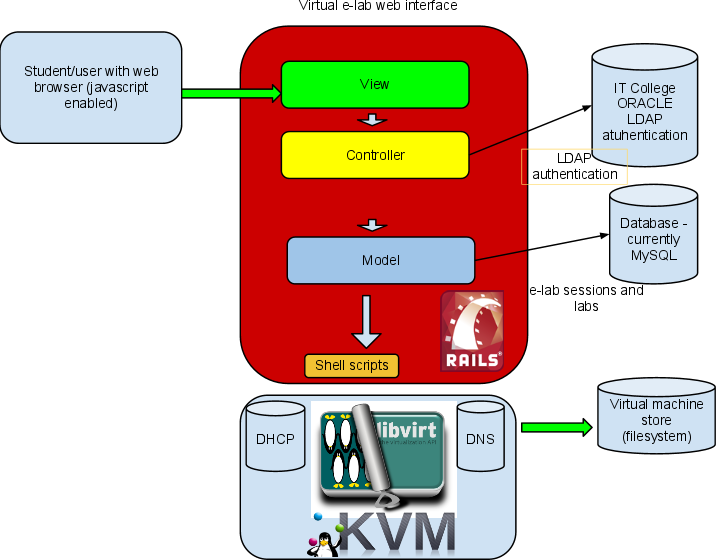
\includegraphics[width=0.8\textwidth]{architecture.png}
\caption{Architecture of Distance Laboratory}
\label{fig:Architecture of Distance Laboratory}
\end{figure}

To support new ideas from this thesis the following development has to be done:
\begin{itemize}
\item implementing a scoring table with virtual reward badges;
\item implementing a new  network configuration infrastructure to support several internal networks isolating \gls{DOS} attacks generated by the students and the \gls{DHCP} traffic;
\item implementing a automatic feedback system for students achievements  in defensive labs.
\end{itemize}

The development is not finished except for the network configuration part. Most of the programming work was done by students as diploma or master projects and supervised by author of this thesis.

The source code of the distance laboratory system is publicly available in a \gls{git} repository~\footnote{The distance laboratory system i-tee -- \url{https://github.com/magavdraakon/i-tee}}.
The system itself is accessible using a \gls{EITC} account~\footnote{The i-tee distance laboratory system -- \url{https://elab.itcollege.ee/}}.
%\subsubsection{New developments for distance study environment}
%
%\begin{itemize}
%	\item normal traffic generator
%	\item malicious traffic generator
%	\item availability monitor (for grading)
%\end{itemize}

\subsection{Operating Systems used in labs}

According to the requirement established in the analysis, the labs should use open source operating systems.
Several operating systems are being used in labs to maintain diversity and avoid vendor locking.
Lab materials are developed with Ubuntu LTS in mind, because of its support and popularity. To get graded the student should choose one different system for defence in at least one lab. The system could be chosen from the following list: OpenBSD, FreeBSD, OpenSolaris, Debian GNU/Linux, Fedora, CentOS, Oracle Linux, OpenSuse. The only restriction is that the chosen system should use a different packaging. For example if a student chooses Ubuntu to do the \gls{DNS} lab then for the \gls{DHCP} lab a operating system without debian packaging system should be used.

Labs with offensive parts are done using Kali GNU/Linux distribution but students can also choose BackTrack.

The main reason the choice is left open is that in labs each student must demonstrate skills and knowledge according to the learning objectives that are more important than knowledge of one system.

\subsection{Choosing software for Root Services lab}
The Root Services labs contains \gls{NTP}, \gls{DNS} and \gls{DHCP} services. However, for fulfilling the learning objectives the software should work on the chosen lab platform -- GNU/Linux Ubuntu Server. 

\subsubsection{The Network Time Protocol server}
Possible choices for \gls{NTP} server software are \emph{OpenNTPD}~\footnote{OpenNTPD \url{http://www.openntpd.org/}
} from OpenBSD  project and the Network Time Protocol Distribution \emph{ntpd} from  Internet Systems Consortium \gls{ISC}~\footnote{Network Time Protocol Distribution \url{http://support.ntp.org/}}. Both packages are installable from ubuntu repositories using the \emph{apt-get} command. The Network Time Protocol Distribution are stored in the main ubuntu repository but OpenNTPD is from the universe section. Therefore the \gls{ntpd} is  slightly more supported by Ubuntu developers.
However, the OpenNTP is designed to be a free, simple and secure implementation of the \gls{NTP} protocol. The \gls{ISC}'s \emph{ntpd} software is free, \gls{IETF} standard compliant and from main/net repository~\footnote{Information from \emph{apt-get show ntp} and \emph{apt-get show openntpd}}. Therefore the \emph{ntpd} daemon was chosen for \gls{NTP} lab.
\subsubsection{The Domain Name System server}
Several \gls{DNS} servers can be used in the lab such as: MaraDNS~\footnote{ MaraDNS is open source, lightweight \gls{DNS} server -- \url{http://www.maradns.org/}}, PowerDNS~\footnote{PowerDNS an open source feature rich \gls{DNS} server -- \url{https://www.powerdns.com/}}, Unbound~\footnote{Unbound is a validating, recursive, and caching \gls{DNS} resolver -- \url{http://unbound.net/}}, NSD~\footnote{NSD is an authoritative only, high performance, simple and open source name server - \url{http://www.nlnetlabs.nl/projects/nsd/}} and \gls{BIND}, because of installation can be done using standard packages from Ubuntu GNU/Linux repositories\footnote{Ubuntu packages --  \url{http://packages.ubuntu.com/}}.

Several \gls{DNS} implementations are not considered for lab, because they lack support for recursive queries or  were designed to be caching only name servers. However, the current \gls{DNS} lab is not using the \gls{DNSSEC} standard, its support is needed for future improvements. Therefore the unbound, NSD and \gls{BIND} are possible choices that are installable from the Ubuntu package repositories. The NSD is suitable for building authoritative (only) servers and can not be used in a \gls{DNS} lab alone.
However, the unbound with NSD or \gls{BIND} alone is suitable for this lab. The \gls{BIND} name-server has a wider user base and a number of installations~\footnote{The \gls{ISC} \gls{BIND} -- \url{https://www.isc.org/software/bind}}. Therefore, the \gls{BIND} name server was chosen for this lab.


\subsection{Choosing software for lab: Protecting Web Application Against (D)DOS Attacks}

\subsubsection{Web server}
According to Netcraft Web Server Survey (May 2013) the web server shares of active websites are: Apache~\footnote{Apache \gls{HTTP} server -- \url{http://projects.apache.org/projects/http_server.html}} -- 55.07\%,  nginx~\footnote{nginx is an HTTP and reverse proxy server -- \url{http://nginx.org/en/}} -- 13.27\%	, Microsoft Internet Information Server~\footnote{Microsoft Internet Information server -- http://www.iis.net/} -- 11.08\% \citep{website:netcraft_web}. Microsoft IIS does not qualify because it is not open source software.  Therefore, the apache is chosen as the primary web server for the lab because of its market share. However, the NGINX is also a important platform and will be used for \gls{TLS} termination in the lab, because students should be able to configure \gls{HTTPS} as well.

\subsubsection{Caching web application acceleration server}
Web acceleration servers are used to reduce the load on the web server and as a mitigation method for small grade denial of service attacks. Is is a possible solution in case of a small attack traffic, but it is useless when all network capacity is occupied by the attack. 
Several popular web application acceleration and caching servers are: Varnish Cache~\footnote{Varnish is a web application accelerator -- \url{https://www.varnish-cache.org}}, NGINX~\footnote{Nginx is an HTTP and reverse proxy server -- \url{http://nginx.org/en/}}, Squid~\footnote{Squid is a caching proxy for the Web -- \url{http://www.squid-cache.org/}}.
The personal cache systems, non open source systems and hardware acceleration systems are not compared because of license or technical limitations.
Even though, the Squid and Nginx are usable for web application acceleration, the Varnish Cache has its own configuration language, giving it an advantage for custom filtering. Therefore, the Varnish Cache was chosen for this lab.

\subsubsection{Web application for testing the web acceleration}
The list of different web applications is long and makes it difficult to give a reasonable choice.
Some applications are common and suitable for load testing and web acceleration for example: WordPress~\footnote{WordPress is open souce website or blog engine -- \url{http://wordpress.org/}}, MediaWiki~\footnote{MediaWiki is open source wiki package -- \url{http://www.mediawiki.org/wiki/MediaWiki}} and  Drupal~\footnote{Drupal is an open source content management platform -- \url{http://drupal.org/}}. Even though, the students can choose their own web application from the previous list, the lab guide covers WordPress because of its easy installation and good documentation.


\subsection{Choosing a vulnerable web application for Protecting an Insecure Web Application lab}

The main need for a vulnerable web application comes from the scenario: Each student installs a vulnerable system and must stop basic attacks without reprogramming a web application.

Although, ready made virtual appliances can be used to install a vulnerable web application the
system administrator should be able to install it himself, helping him to understand the main architecture of a web application to choose suitable protection methods. Therefore, the chosen application should be free and open source, easily installable, implementing  at least stored and reflected \gls{XSS}, several injection type attacks like \gls{SQLi} (usual and blind) and \gls{CSRF}.

\subsubsection{WebGoat}
WebGoat is a free, open source insecure J2EE web application designed to teach web application security lessons~\footnote{WebGoat -- \url{https://www.owasp.org/index.php/Category:OWASP_WebGoat_Project}}.  Even though, the WebGoat is one of the best applications for teaching web vulnerabilities, the installation and J2EE requirement is not suitable for system administration students because it has too many steps to follow.


\subsubsection{Damn Vulnerable Web Application}
The Damn Vulnerable Web Application \gls{DVWA} is web application with several vulnerabilities. It is suitable for testing several security vulnerabilities and tools. Even though, the tool does not implement all \gls{OWASP} top ten attacks, the most relevant are presented. The tool is written using PHP/MySQL which are taught to all \gls{EITC} students and usually known by system administrators. The tool is designed for learning and students can choose the difficulty level of exploiting~\citep{website:dvwa}.

The program is easy to install. It has integrated study materials and variable levels of vulnerabilities.
The vulnerability coverage is not best compared to WebGoat but is sufficient for this lab.

\subsubsection{NOWASP (Mutillidae)}
NOWASP (Mutillidae)~\footnote{NOWASP (Mutillidae) -- \url{http://sourceforge.net/projects/mutillidae/}} web pen-test practice application is a free, open source vulnerable web-application for labs, security enthusiasts, classrooms, \gls{CTF}, and vulnerability assessment tool targets. \citep{website:Mutillidae} Although, the tool documentation has videos, study materials and a good support for \gls{OWASP} top ten vulnerabilities, but the development relies on one person and the community support is thin.
\subsubsection{SQLol}
SQLol~\footnote{SQLol -- \url{https://github.com/SpiderLabs/SQLol
}} is a free and open source web application designed to test \gls{SQLi} type attacks and is compatible with \gls{MySQL}, gls{PostgreSQL}. Even though, the application has comprehensive capabilities on \gls{SQLi}, the other vulnerabilities are not covered.


In conclusion, because of the defensive nature of the developed course, only simple vulnerabilities are needed to demonstrate a problem and all vulnerable applications are suitable for the lab. To create diversity all the applications that can be installed easily may be used in the lab. All the examples are given using \gls{DVWA} (because of its name) but to get the grade every student should choose another vulnerable application from the list, install  and protect it.

{\color{red} Siin on pooleli}
\subsection{Web application firewall and database firewall}


According to lab scenario the \gls{SQLi} attacks should be stopped before database (Appendix~\ref{Protecting an Insecure Web Application}). Several proprietary database firewall products like Oracle Audit Vault and Database Firewall and SecureSphere Database Firewall can provide functionality needed. However, they are not applicable in this lab because they are not free and open source software products.

Only functional open source database firewall with enterprise scale functionality like web based administrative interface, support for different databases and easy to use for database administrator was GreenSQL open source database firewall. However, the development of this version is stopped and now even download is not possible from vendor homepage~\footnote{GreenSQL -- http://www.greensql.com/}, the source files and pre-build packages for Ubuntu Server 12.04 LTS 64bit are downloadable from \gls{EITC} lab page~\footnote{\gls{EITC} fork of GreenSQL database -- \url{http://elab.itcollege.ee:8000/Day3/}}. Moreover the author of this thesis fixed the source code of the firewall to get it compile with newer GNU/C compiler.

For learning basics of the database fire-walling the enterprise products are not needed and for this lab open source version of GreenSQL database firewall was chosen.

However, the free closed source version is still downloadable from vendor homepage, the future work is find open source replacement for GreenSQL which is actively developed and has comparable functionality.

The database firewall provides protection only for database but for example the reflected \gls{XSS} are not seen in database layer. Therefore, this protection is not sufficient and additional filtering in web layer is needed and Web Application Firewall \gls{WAF} to be integrated into lab scenario.

The common open source \gls{WAF} is ModSecurity~\citep[p.196]{book:practica_intrusion_analysis} from Trustwave SpiderLabs~\footnote{Trustwave SpiderLabs -- \url{https://www.trustwave.com/spiderlabs/}}. However, the ModSecurity itself is a parsing/blocking engine and needs proper rule set to block/log attacks, like \gls{OWASP} Core Rule Set Project~\footnote{OWASP ModSecurity Core Rule Set Project -- }. However, some alternatives exists and ModSecurity rules are too hard to modify for students in authors opinion the \gls{EITC} partners and several companies in Estonia using it according to conversations and discussion between system administrators from pilot lab. The product supports apache, Enginx and Inernet Information Server web servers~\footnote{Mod Security overview -- \url{http://www.modsecurity.org/projects/modsecurity/index.html}} and compatible with web servers chosen to this lab.

Therefore, the Mod Security and \gls{OWASP} Core Rule Set was chosen for this lab.



\section{Development of the e-learning course}
After choosing technological tools the lab materials need to be created~\citep{OppeArenduskeskus2010}. Therefore, the course materials are created, reviewed and run-through by small test group.

\subsection{Authoring the learning material}
Developing learning material is based on learning objectives. Each learning objective must be covered with learning material and everything else should left out as extra load for student. Therefore in the development phase the authoring of different study materials, assessment tests, audio/video media and integration of all artefacts into consistent body with one reason: ensure that all objectives are met.

Authoring the study materials is one of most time consuming tasks and amount of developed study materials is too big even for appendices. Therefore one sample block - Securing web applications are included in Appendix~\ref{Protecting Web Application Against (D)DOS Attacks} and in Appendix~ \ref{Protecting an Insecure Web Application} 

Developed learning material are publicly available and under (\gls{CC-BY-SA}) license to guarantee maximum impact on field. Therefore is acceptable that people with will and motivation may self-study using this e-learning course. Moreover, the private training companies can use those courses to train target group.

Learning materials, self-tests, course information and other materials are publicly downloadable~\footnote{\href{http://elab.itcollege.ee:8000/cyber-course/}{Course Syllabus (Õpijuhis)}}.


Some never materials are developed using open source revision control system \gls{git} and all changes and commits are publicly available. Moreover, source code of this thesis and labs are available from public \gls{git} repository with \LaTeX  source files and as well other files~\footnote{\href{https://github.com/magavdraakon/margus-thesis.git}{Materials and source code of this thesis}}.


Developed learning material should follow consistent style and present also one example of good documentation practice. For system administrators several howto styles exists. However practical hands-on laboratory instructions are designed that pass through using copy paste is possible but gives one working sample. However, this is not enough to pass lab scenario and student must customize own configuration.

Guiding stile of the lab instruction using style convention: First, all variable parts of the text are clearly differs from other text and command. Second, all commands given by student are highlighted, and variable parts embossed as seen in followed command.


\begin{minted}[frame=lines,framesep=2mm]{bash}
#For changing Out of memory - OOM adjustment score for mysql server
echo "-1000" > /proc/$(pidof mysqld)/oom_score_adj
\end{minted}
%$



Sample sample: Finding a proccess ID of the mysql server proccess.

\begin{minted}[frame=lines,framesep=2mm]{bash}
ps -ef|grep mysqld
\end{minted}
\label{code_sample}
%
\small{
\begin{Verbatim}[samepage=true,frame=single,
label=Command output,framesep=2mm,rulecolor=\color{red},commandchars=\\\{\}]
sudent@opiise:~# ps -ef|grep mysqld
root     11290 10905  0 10:27 pts/6    00:00:00 grep --color=auto mysqld
mysql    \fbox{\color{red}29830}    1  0 Apr25 ?        00:05:47 /usr/sbin/mysqld
\end{Verbatim}
%
}

All study should stored in open formats, like pdf, OpenDocument, MediaWiki markup language, html, utf8 text. Original editable source files for generating pdf, images should be publicly accessible. Moreover, text based materials should stored into version control system like \gls{git} to enable contributing for other lecturers and students as well.

%
%
%\begin{table}[H]
%\centering
%\caption{The learning materials}
%
%\begin{tabular}{|p{5cm}|p{3cm}|p{6cm}|}
%\hline 
%\color{blue}
%Name & \color{blue} Comments  & \color{blue} Location \\ 
%
%\hline
%  \multicolumn{3}{|c|}{Pre-requirement course} \\
%\hline
%Operating system basics & & \\
%\hline
%Basic networking IPv4/IPv6, TCP/IP & & \\
%
%\hline
%GNU/Linux basics  & & \\
%\hline
%Scripting in BASH &  & \\
%\hline
%Scripting in Python & Co authored with Lauri Võsandi & \\
%\hline
%Scripting in PowerShell & Author is Heiki Tähis & \\
%
%
%\hline
%\hline
%  \multicolumn{3}{|c|}{Root services} \\
%
%\hline 
%
%
%Lecture - Configuring NTP service & (Estonian 2012), Learning outcome no XXX & \url{http://goo.gl/toRpw} \\ 
%\hline 
%Practical class - Configuring NTP in Ubuntu  & (Estonian 2012), Learning outcome no XXX , Students improved & \url{https://wiki.itcollege.ee/index.php/NTP_Ubuntus} \\
%\hline 
%Lecture DNS & & \href{http://enos.itcollege.ee/~mernits/infrastruktuur/Interneti%20domeeninimede%20s%c3%bcsteem%20-%20IT%20infra%20loeng.odp}
%{DNS Lecture [OpenDocument]} \\
%\hline
%Practical class - DNS & Co authored with Katrin Loodus  & \href{https://docs.google.com/document/d/1ZeQpPXdVq1C7RQpxQYR0gBB0OBMYB_0g6aFFxs_-fIA/edit}{Configuring DNS [GoogleDocs] } \\
%
%\hline
%\hline
%  \multicolumn{3}{|c|}{Web/File Services} \\
%
%\hline 
% & & \\
%\hline
%
%\hline
% & & \\
%\hline
%\hline
%
%\end{tabular} 
%\label{table:learning_materials}
%\end{table}


\subsection{Course Syllabus}
\label{Course Syllabus}
The participant of the course will get first information from Course Syllabus, where all relevant information about the course must be listed as: list of learning materials, course schedule, list of the labs, list of topics, list of exercises and homework, deadlines, grading information. Course Syllabus will be in \gls{EITC} study information system but the public copy of the information is available from lab website~\footnote{Course Syllabus -- \url{http://elab.itcollege.ee:8000/cyber-course/}}

\subsection{Testing the e-course}
Before experimenting with students in larger group the all course modules got tested by co-workers -- lecturers and assistants of \gls{EITC}. After in-house testing each lab run-through by small group of system administrator from different organizations including \gls{EISA}. Evaluation summary for the course is in Table~\ref{table:desing_develop_evaluation}.
\begin{table}[h]
\centering
\caption{The evaluation of the design and development stage }
{ \small 
\begin{tabular}{|p{6cm}|p{2cm}|p{5cm}|}
\hline 
\color{blue} Evaluation question & \color{blue} Result [1..4] & \color{blue} Comments and references \\
\hline
Does course have a proper structure? 
& 4  &  Course Syllabus has links for study program, topics and labs  \\ 
\hline
Does chosen presentation learning material support the learning outcomes of the course? 
& 4  &  Active participation of the students are encouraged \\ 
\hline

Do the learning materials follow best practices? 
& 3  &  Some materials needs improvement \\ 
\hline
Is all web material available? 
& 4  &  Materials are in course syllabus page \\ 
\hline
Does sufficient course syllabus exists? 
& 4  &  Course Syllabus are in course web page \\ 
\hline 
Does student needs non-free software for participation?
& 4 &  No, all software used is open source (except PowerShell lab where sotware are provided by \gls{EITC}) \\ 
\hline 
Is course tested before including to the curriculum?
& 4 & Course is tested using 22 students and >80 system administrators \\ 
\hline
Does course technically work (links, materials)?
& - & Testing is not completed, because migrating to the distance study environment. In case on this course there much more to be tested than links, for example all virtual machines.\\ 
\hline 
\end{tabular} 
}
\label{table:desing_develop_evaluation}
\end{table}


\section{Implementation of the e-learning course}

In the implementation phase, the courses are piloted and feedback from students and other lecturers are gathered also a arranging the learning space and time and preparing learners for the course~\citep{OppeArenduskeskus2010}.

Author of this thesis piloted each block of the course and collected feedbacks from the students, make notes with improvement ideas and motivated students to behave as active and motivated as possible.
First lab was relatively simple because of simplicity of the topic -- \gls{NTP} compared for example web server lab. However, this was intentional because during this lab the technical details are explained to the students about virtualization environment and roles of lecturer and students in this course. Therefore slow start is important for students to learn environment and organizational aspects of the course. Thereafter, a studies went smoothly for students with proper prerequisite skills and knowledge and hard for others. The main thing learned from implementation: This course is too hard for most of the students but the are motivated to learn the content. However, the preliminary course is mandatory for most of the students and system administrators because small group of students with inadequate level may slow down a whole class. During the implementation phase the piloting course was evaluated using self-assessment and criteria from \gls{ADDIE} model~\citep{OppeArenduskeskus2010}. The results are presented in Table~\ref{table:implementation_evaluation}.

\begin{table}[h]
\centering
\caption{The evaluation of the implementation stage }
{ \small 
\begin{tabular}{|p{6cm}|p{2cm}|p{5cm}|}
\hline 
\color{blue} Evaluation question & \color{blue} Result [1..4] & \color{blue} Comments and references \\ 
\hline
Students are motivated to be active? 
& 4  &  Active participation of the students are encouraged \\ 
\hline 
Does lecturer give feedback to the students?
& 4 &  Students will get immediate feedback during contact classes, students know that \\ 
\hline 
Did lecturer collect data during the course how to improve course in the future?
& 3 & Data is collected but not yet implemented (will be in next course) \\ 
\hline
Does feedback from student collected?
& 4 & After every course and training feedback are collected. \\ 
\hline 
\end{tabular} 
}
\label{table:implementation_evaluation}
\end{table}

